\section{Deep Structured Prediction in NLP}
\label{sec:background:deepsp}
Due to the power of representation learning, deep learning is widely
used to extract sophisticated representations for the inputs in
various NLP tasks. In this thesis, instead of focusing on a single
task, we systematically study the representation learning challenges
for multiple sets of tasks based on independent factorization
assumption.  In this section, We summerize the recent advances in deep
structured prediction with respect to representational
formalism~\S\ref{ssec:bg:formalism},
learning~\S\ref{ssec:bg:rep-learning} and
inference~\S\ref{ssec:bg:inference} respectively.

In this thesis, we study the specific inductive biases based on the
principle of compositionality, which can be used for \textbf{different
  purposes more than the accuracy on a single task or a single
  domain}. For example, with simple independent factorization, we
study a universal alignment-based model to support
\textit{cross-framework} meaning representation parsing. By defining
two complementary dialogueue observers to sequentially predict the
MISC code for both current and future utterance, our model emphasizes
both \textit{accurate and real-time} assistance to a therapist. We
propose to represent the output labels with natural language
descriptions for \textit{zero-shot learning} on unseen
labels~\S\ref{ssec:sgdst}. In our thesis, we show that during the
rapid progress of representation learning methods, our proposed
inductive biases still can outperform the standard usage baselines.

\subsection{Formulation of Structural Interdependence}
\label{ssec:bg:formalism}

\Paragraph{Graphical Models} A graphical model is a probabilistic
model for which a graph expresses the conditional dependence structure
between random variables. Generally, probabilistic graphical models
use a graph-based representation as the foundation for encoding a
distribution over a multi-dimensional space, which represents a set of
independences that hold in the specific distribution. Two branches of
graphical representations of distributions are commonly used, namely,
Bayesian networks and Markov random fields. Both families encompass
the properties of factorization and independences, but they differ in
the set of independences they can encode and the factorization of the
distribution that they induce.  In this thesis, we mainly use the
undirected Markov random fileds to represent our independent
factorization assumptions.

As shown in~\autoref{fig:bg:graphical-model}, each circle represent a
variable, while each rectangle shows a factor between the input
sentence variable $x$ and each decomposed segements of output
structures $y$. The difference between left and right figure lies to
the alignment variable $a$ in the center. In the left figure, the
shade cicle $a$ means the alignment are explicitly observed after the
decomposion. While in the right figure, the alignment variable $a$ is
not observed.

\begin{figure}[!th]
\centering
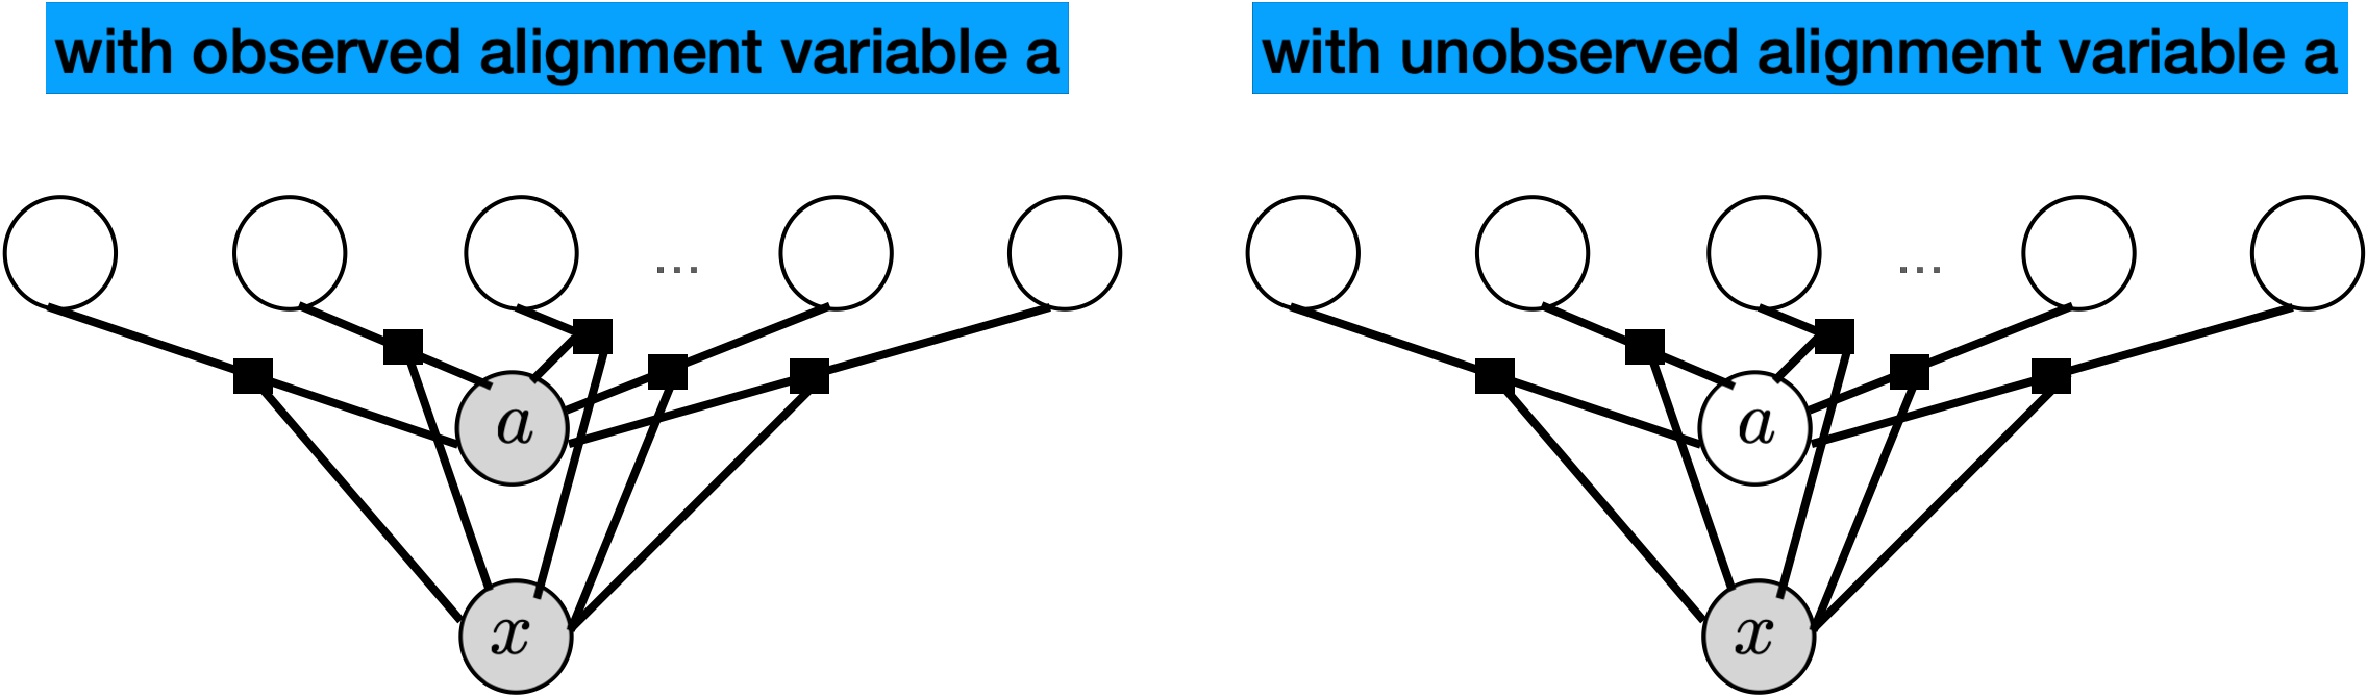
\includegraphics[width=0.90\textwidth]{graphical-models.pdf}
\caption{\label{fig:bg:graphical-model}The factor representation for
  the independent factorization used in our thesis}
\end{figure}

\Paragraph{Constrained Conditional Models} Besides using graphical
models to declaritively represent the structural interdependence
between variables, constrained conditional
models~\citep[CCM,][]{chang2012structured} is another machine learning
and inference framework for the same goals. More specifically, CCM
emphasizes augmenting the learning of conditional models with
declarative constraints. It aims to support constrained decisions in
an expressive output space while maintaining modularity and
tractability of training and inference. These constraints can express
either hard restrictions, completely prohibiting some assignments, or
soft restrictions, penalizing unlikely assignments. One popular
formalism to represent the constraints is to use an interger linear
programming~(ILP), which has been widely used to constrain learning in
many NLP tasks~\citep{roth2007global}. The declaritive linear
objective functions and linear constraints, and the availibities of
the off-the-shelf solvers make this formalism very easy to use.

Recently, to inject known hand-crafted constraints bewteen discrete
variable assignments in the deep neural networks, one foundmental
challange is how to represent the constraints in end-to-end
differentiable ways~\cite{bach2017hinge}. For example,
\citet{li2019augmenting} propose to use differentiable fuzzy logic
operators to augment the neural networks with boolean
logic. \citet{pacheco2021modeling} introduces a declarative Deep
Relational Learning framework~(\DRAIL) via integrating neural
representation learners with probabilistic logic.

Besides representing the constraints as logic forms, many recent work
also studies representing constraints with discrete latent variable
models, such as StructVAE for latent tree structured variables,
~\cite{yin2018structvae, corro2019learning}. Our work on latent
alignment models also falls into this category.

Besides injecting declaritive constraints, recent research also learn
the constraints in an end-to-end
ways. \citet[SPEN,][]{belanger2016structured} define energy functions
that can learn the arbitrary dependencies among parts of structured
outputs by relaxing the whole structured outputs into continuous
vectors, Following this, inference network~\cite{tu2018learning} was
proposed to learn the constrained network for inference, which
approximate the cost-augmented inference during training and then
fine-tuning for test-time inference.

\subsection{Neural Representation Learning}
\label{ssec:bg:rep-learning}
For deep learning based methods, we review the recent advances from
static word embedding based methods to attention-based dynamic
features selection and contextualized representation. Finally, we also
introduced the rapid progress in language encoding architectures, from
recurrent neural network to transformer, and the corresponding
pretrained language models ELMo , BERT, GPT3 etc.

\Paragraph{Static Word Embedding}


\Paragraph{Contetualized Representation and Contextualing Models}



\subsection{Inference}
\label{ssec:bg:inference}
\subsubsection{MAP Inference}
Exact: Dynamic Programming: Viterbi, CKY, Max Spanning Arborescence, Exact Search, Integer Linear Programming
Approximate: Sampling, Beam Search/Learning to Search, Linear Programming Relaxations

\subsubsection{Marginal Inference}
Forward-Backward/ Inside-outside/ Matrix tree
CRF
SparseMAP

%%% Local Variables:
%%% mode: latex
%%% TeX-master: "../../thesis-main.ltx"
%%% End:
